\chapter{Chromatographie}\label{ch:b2:chromatography}

Une goutte de boisson énergisante, diluée et filtrée, est injectée dans un tube d'acier pas plus long
qu'un stylo, rempli de grains de silice de quelques micromètres. Quelques minutes plus tard, un
détecteur a tracé une ligne portant une poignée de pics, et à partir de l'aire de l'un d'eux le
laboratoire indique la quantité de caféine que contient la canette, à quelques pour cent près. La
\omterm{def:b2:chromatography:principle}{chromatographie} sépare les constituants d'un mélange en les faisant courir dans une colonne à des
vitesses différentes~; ce chapitre explique pourquoi ils se déplacent à des vitesses différentes,
pourquoi leurs pics ont la largeur qu'ils ont, comment séparer deux voisins, et comment transformer un
pic en une quantité.

\begin{omfigure}
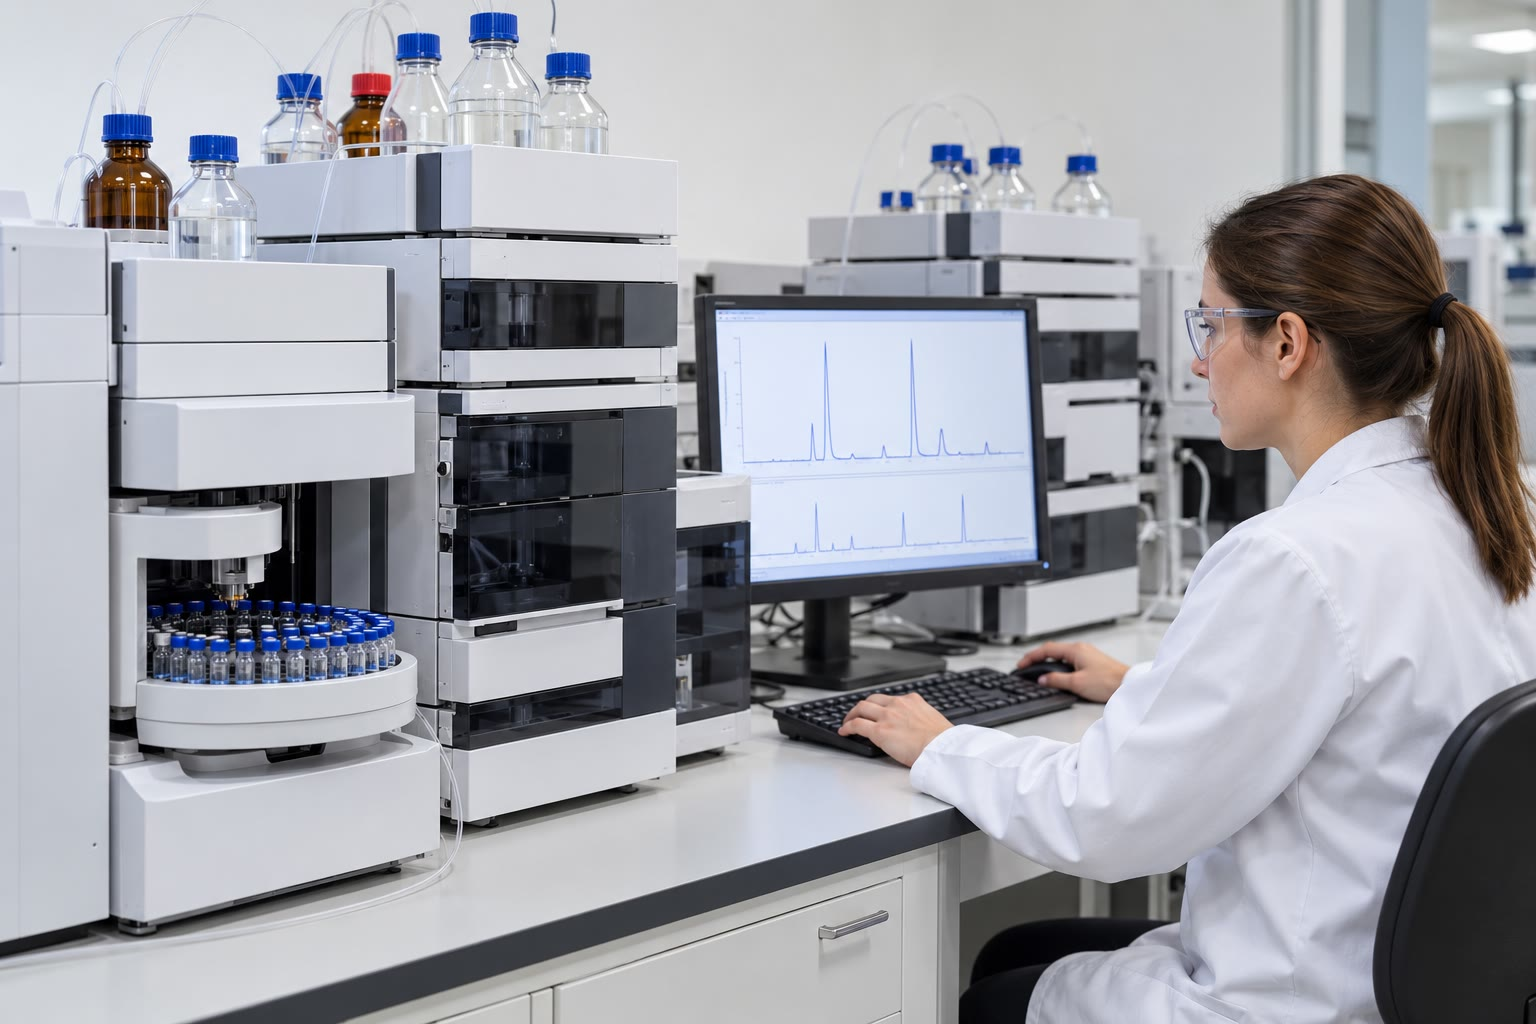
\includegraphics[width=0.58\linewidth]{images/book3/ai/b2-31-analytical-lab.jpg}

{\small Un laboratoire d'analyse~: des chromatographes en phase liquide avec leurs flacons de solvant et
un plateau d'échantillonneur automatique garni de flacons~; les chromatogrammes s'affichent à l'écran (illustration).}
\end{omfigure}

\begin{recall}
Le volume scolaire~: \omterm{def:b2:chromatography:principle}{chromatographie} sur papier et sur couche mince, chromatogramme, éluant. Le volume
de première année~: coefficient de partage, extraction liquide--liquide, rapport frontal $R_f$ d'une
plaque de \omterm{def:b2:chromatography:principle}{chromatographie} sur couche mince. \Cref{ch:b2:liquid-vapour-diagrams}~: le \omterm{def:b2:liquid-vapour-diagrams:fractional-distillation}{plateau théorique}
d'une colonne de distillation.
\end{recall}

\section{Principe}

\begin{definition}[Chromatographie]\label{def:b2:chromatography:principle}
La \emph{chromatographie}\index{chromatographie} sépare les constituants d'un mélange en les répartissant
entre une \emph{phase stationnaire}\index{phase stationnaire}, fixée dans une colonne ou sur une plaque, et
une \emph{phase mobile}\index{phase mobile}, gaz ou liquide qui s'écoule à son contact. L'entraînement des
constituants à travers la colonne, puis hors de celle-ci, par la phase mobile est l'\emph{élution}\index{elution@élution}.
\end{definition}

Une molécule n'avance que lorsqu'elle se trouve dans la \omterm{def:b2:chromatography:principle}{phase mobile}~; quand elle est retenue par la \omterm{def:b2:chromatography:principle}{phase
stationnaire}, elle attend. Elle passe d'une phase à l'autre des millions de fois sur son trajet, si bien
que sa vitesse moyenne est fixée par la fraction du temps qu'elle passe dans chacune, c'est-à-dire par
son équilibre de partage.

\begin{definition}[Rétention]\label{def:b2:chromatography:retention}
Le \emph{temps de rétention}\index{temps de retention@temps de rétention} $t_R$ d'un composé est la durée
qui sépare l'injection du maximum de son pic~; le \emph{temps mort}\index{temps mort} $t_M$ est le temps
de rétention d'un composé non retenu, qui n'entre jamais dans la \omterm{def:b2:chromatography:principle}{phase stationnaire}. Le \emph{facteur de
rétention}\index{facteur de retention k@facteur de rétention $k$}
$k$ d'un composé sur une colonne vaut
\begin{equation*}
k = \frac{t_R - t_M}{t_M}.
\end{equation*}
Ce n'est pas le $R_f$ d'une plaque de \omterm{def:b2:chromatography:principle}{chromatographie} sur couche mince, qui mesure une distance
parcourue, bien que tous deux décrivent le même partage.
\end{definition}

\begin{proposition}[Temps de rétention]\label{prop:b2:chromatography:retention-time}
Si, à l'équilibre, les quantités d'un composé dans les \omterm{def:b2:chromatography:principle}{phases stationnaire} et mobile d'une tranche de
colonne valent $n_s$ et $n_m$, le composé avance à la vitesse $u/(1 + n_s/n_m)$, où $u$ est la vitesse de
la \omterm{def:b2:chromatography:principle}{phase mobile}, et $t_R = t_M(1 + n_s/n_m)$.
\end{proposition}

\begin{proof}
Une molécule donnée passe la fraction $n_m/(n_s + n_m)$ de son temps dans la \omterm{def:b2:chromatography:principle}{phase mobile}, où elle avance
à la vitesse
$u$, et le reste à l'arrêt. Sa vitesse moyenne vaut $u\,n_m/(n_s + n_m) = u/(1 + n_s/n_m)$. La colonne de
longueur $L$ est traversée en $t_R = (L/u)(1 + n_s/n_m)$, et $L/u = t_M$.
\end{proof}

\begin{proposition}[Rétention et partage]\label{prop:b2:chromatography:k-and-K}
Le \omterm{def:b2:chromatography:retention}{facteur de rétention} est le rapport des quantités dans les deux phases, $k = n_s/n_m = KV_s/V_m$, où $K$
est le coefficient de partage (concentration dans la \omterm{def:b2:chromatography:principle}{phase stationnaire} sur concentration dans la \omterm{def:b2:chromatography:principle}{phase
mobile}) et $V_s$, $V_m$ les volumes des phases dans la colonne.
\end{proposition}

\begin{proof}
D'après la \cref{prop:b2:chromatography:retention-time}, $(t_R - t_M)/t_M = n_s/n_m$. Avec $n_s = c_sV_s$,
$n_m = c_mV_m$ et $K = c_s/c_m$, $n_s/n_m = KV_s/V_m$.
\end{proof}

Deux composés se séparent si leurs coefficients de partage diffèrent~; la géométrie de la colonne
($V_s/V_m$) multiplie toutes les rétentions de la même façon. Changer la \omterm{def:b2:chromatography:principle}{phase mobile}, ce qui modifie $K$,
est le principal levier du chimiste sur la rétention.

\begin{omfigure}
\begin{tikzpicture}[x=1cm, y=1cm]
\foreach \x/\a/\b/\ha/\hb/\lab in {0/0.6/0.6/0.1/0.1/début, 2.4/1.5/2.6/0.16/0.22/plus tard, 4.8/2.4/4.4/0.2/0.3/fin}{
  \draw[black!60] (\x-0.35,0) rectangle (\x+0.35,-5);
  \fill[omThm!55] (\x-0.33,-\b+\hb) rectangle (\x+0.33,-\b-\hb);
  \fill[omDef!55, opacity=0.85] (\x-0.33,-\a+\ha) rectangle (\x+0.33,-\a-\ha);
  \node[font=\small] at (\x,-5.4) {\lab};
}
\draw[->, thick] (-1.0,-0.3) -- (-1.0,-4.6) node[midway, left, font=\small, align=right] {phase\\mobile};
\node[font=\small, align=left, anchor=west] at (5.5,-2.4) {plus retenu\\(lent, étroit)};
\node[font=\small, align=left, anchor=west] at (5.5,-4.4) {moins retenu\\(rapide)};
\draw[densely dotted] (5.15,-2.4) -- (5.5,-2.4); \draw[densely dotted] (5.15,-4.4) -- (5.5,-4.4);
\end{tikzpicture}
\par\vspace{4pt}

{\small Deux composés injectés ensemble sous forme d'une bande mince descendent une colonne (trois
instantanés, schématique). Le moins retenu ($k$ plus petit) prend de l'avance~; les deux bandes
s'élargissent au cours de leur trajet, d'autant plus qu'elles sont allées plus loin.}
\end{omfigure}

\section{Largeur des pics et nombre de plateaux}

Une bande ne reste pas mince. Les molécules d'un même composé empruntent des chemins différents entre les
grains, diffusent le long de la colonne et prennent dans la \omterm{def:b2:chromatography:principle}{phase stationnaire} des retards aléatoires. Le
pic enregistré à la sortie est très proche d'une gaussienne d'écart type $\sigma_t$ (en temps), et plus
il est étroit pour un $t_R$ donné, meilleure est la colonne.

\begin{definition}[Nombre de plateaux]\label{def:b2:chromatography:plates}
Le \emph{nombre de plateaux théoriques}\index{nombre de plateaux theoriques@nombre de plateaux théoriques} d'une
colonne pour un composé vaut $N = (t_R/\sigma_t)^2$, où
$\sigma_t$ est l'écart type de son pic en temps. La \emph{hauteur équivalente à un plateau
théorique}\index{hauteur equivalente a un plateau theorique@hauteur équivalente à un plateau théorique} vaut
$H = L/N$, pour une colonne de longueur $L$.
\end{definition}

Ces noms viennent de la colonne de distillation du \cref{ch:b2:liquid-vapour-diagrams}~: une colonne
chromatographique se comporte comme si elle était un empilement de $N$ étages d'équilibre, chacun de
hauteur $H$. L'analogie est une façon de compter, non une image de la colonne.

\begin{proposition}[Nombre de plateaux à partir d'un pic]\label{prop:b2:chromatography:plate-number}
Avec $w$ la largeur à la base entre les tangentes aux points d'inflexion et $w_{1/2}$ la largeur à
mi-hauteur,
\begin{equation*}
N = 16\left(\frac{t_R}{w}\right)^2 = 5.54\left(\frac{t_R}{w_{1/2}}\right)^2.
\end{equation*}
\end{proposition}

\begin{proof}
Pour une gaussienne d'écart type $\sigma$ et de hauteur $h$, les points d'inflexion sont en $\pm\sigma$,
où la hauteur vaut $h\mathrm e^{-1/2}$ et la pente $\mp h\mathrm e^{-1/2}/\sigma$~; la tangente en ce
point atteint zéro après $\sigma$ de plus, en $\pm2\sigma$~: $w = 4\sigma$. La mi-hauteur est atteinte là
où
$\mathrm e^{-x^2/2\sigma^2} = 1/2$, $x = \sigma\sqrt{2\ln2}$~: $w_{1/2} = 2\sqrt{2\ln2}\,\sigma \approx
2.355\,\sigma$. Substituer $\sigma = w/4$ ou $\sigma = w_{1/2}/2.355$ dans $N = (t_R/\sigma)^2$ donne
$16$ et $2.355^2 = 5.545$, qu'on écrit 5.54.
\end{proof}

\begin{proposition}[Équation de van Deemter]\label{prop:b2:chromatography:van-deemter}
La \omterm{def:b2:chromatography:plates}{hauteur de plateau} dépend de la vitesse linéaire $u$ de la \omterm{def:b2:chromatography:principle}{phase mobile} selon
\begin{equation*}
H = A + \frac{B}{u} + Cu,
\end{equation*}
où $A$ rend compte des différents chemins à travers le garnissage, $B/u$ de la diffusion le long de la
colonne (plus forte quand les molécules séjournent plus longtemps) et $Cu$ de la lenteur des échanges avec
la \omterm{def:b2:chromatography:principle}{phase stationnaire} (plus gênante quand la \omterm{def:b2:chromatography:principle}{phase mobile} passe vite). $H$ est minimale en $u_{\mathrm{opt}} = \sqrt{B/C}$, où $H_{\min} =
A + 2\sqrt{BC}$.
\end{proposition}

\admitted

La forme de l'équation est admise~; son minimum ne l'est pas. $\mathrm dH/\mathrm du = -B/u^2 + C$ s'annule
en $u = \sqrt{B/C}$, et là $B/u = Cu = \sqrt{BC}$, d'où $H_{\min} = A + 2\sqrt{BC}$~; la dérivée seconde
$2B/u^3$ est positive, il s'agit donc d'un minimum. Des grains fins réduisent $A$ et $C$~: c'est pourquoi
la \omterm{def:b2:chromatography:principle}{chromatographie} liquide moderne utilise des particules de quelques micromètres et de hautes pressions
pour y faire passer la \omterm{def:b2:chromatography:principle}{phase mobile}.

\begin{omfigure}
\begin{tikzpicture}
\begin{axis}[width=0.7\linewidth, height=5.2cm, xmin=0, xmax=8, ymin=0, ymax=70,
  xlabel={vitesse linéaire $u$ (\unit{mm/s})}, ylabel={hauteur de plateau $H$ (\unit{\micro m})},
  label style={font=\small}, tick label style={font=\scriptsize},
  legend style={font=\scriptsize, at={(1.03,1)}, anchor=north west}, legend cell align=left]
\addplot[omDef, very thick] table[x=u, y=H] {figdata/out/bachelor-2-chromatogram-b.dat};
\addplot[black!50, dashed] table[x=u, y=A] {figdata/out/bachelor-2-chromatogram-b.dat};
\addplot[omThm, dashed] table[x=u, y=B] {figdata/out/bachelor-2-chromatogram-b.dat};
\addplot[omMeth, dashed] table[x=u, y=C] {figdata/out/bachelor-2-chromatogram-b.dat};
\addplot[only marks, mark=*, mark size=1.6pt] coordinates {(2,30)};
\legend{$H$, $A$, $B/u$, $Cu$}
\end{axis}
\end{tikzpicture}

{\small Une courbe de van Deemter (paramètres de l'exercice~: $A = \qty{10}{\micro m}$, $B = \qty{20}{\micro m.mm/s}$,
$C = \qty{5}{\micro m.s/mm}$). Le minimum, $H = \qty{30}{\micro m}$ pour $u = \qty{2}{mm/s}$, se situe là où
les termes de diffusion et d'échange sont égaux.}
% figdata: bachelor-2/chromatogram.py part b
\end{omfigure}

\section{Séparer deux composés}

\begin{definition}[Sélectivité et résolution]\label{def:b2:chromatography:separation}
Pour deux pics voisins avec $k_2 > k_1$, le \emph{facteur de sélectivité}\index{facteur de selectivite@facteur de sélectivité} vaut
$\alpha = k_2/k_1$, et la \emph{résolution}\index{resolution@résolution} vaut
\begin{equation*}
R_s = \frac{2(t_{R2} - t_{R1})}{w_1 + w_2},
\end{equation*}
la distance entre les pics divisée par leur largeur moyenne à la base.
\end{definition}

Pour $R_s = 1$, les pics se chevauchent encore visiblement~; pour $R_s = 1.5$, le signal revient à la
ligne de base entre eux (séparation à la ligne de base), ce qui est l'objectif habituel des dosages.

\begin{omfigure}
\begin{tikzpicture}
\begin{axis}[width=0.36\linewidth, height=3.6cm, xmin=-8, xmax=8, ymin=0, ymax=1.15,
  xtick=\empty, ytick=\empty, axis x line=bottom, axis y line=none, title style={font=\small},
  title={$R_s = 0.75$}]
\addplot[omDef, thick] table[x=x, y=r075] {figdata/out/bachelor-2-chromatogram-a.dat};
\end{axis}
\end{tikzpicture}\hfill\begin{tikzpicture}
\begin{axis}[width=0.36\linewidth, height=3.6cm, xmin=-8, xmax=8, ymin=0, ymax=1.15,
  xtick=\empty, ytick=\empty, axis x line=bottom, axis y line=none, title style={font=\small},
  title={$R_s = 1.0$}]
\addplot[omDef, thick] table[x=x, y=r100] {figdata/out/bachelor-2-chromatogram-a.dat};
\end{axis}
\end{tikzpicture}\hfill\begin{tikzpicture}
\begin{axis}[width=0.36\linewidth, height=3.6cm, xmin=-8, xmax=8, ymin=0, ymax=1.15,
  xtick=\empty, ytick=\empty, axis x line=bottom, axis y line=none, title style={font=\small},
  title={$R_s = 1.5$}]
\addplot[omDef, thick] table[x=x, y=r150] {figdata/out/bachelor-2-chromatogram-a.dat};
\end{axis}
\end{tikzpicture}

{\small Deux pics gaussiens de même taille à trois \omterm{def:b2:chromatography:separation}{résolutions} (modèle). À 0.75, ils se confondent en un
doublet~; à 1.0, la vallée est encore au quart de la hauteur~; à 1.5, le signal est revenu à la ligne
de base.}
% figdata: bachelor-2/chromatogram.py part a
\end{omfigure}

\begin{theorem}[Équation de la résolution]\label{thm:b2:chromatography:resolution}
Pour deux pics voisins de même nombre de plateaux $N$,
\begin{equation*}
R_s = \frac{\sqrt N}{4}\,\frac{\alpha - 1}{\alpha}\,\frac{k_2}{1 + k_2}.
\end{equation*}
\end{theorem}

\begin{proof}
Pour des pics proches, les deux largeurs à la base sont presque égales~; les prendre toutes deux égales à
celle du second pic,
$w = 4\sigma_t = 4t_{R2}/\sqrt N$ (\cref{def:b2:chromatography:plates}). Alors $R_s = (t_{R2} -
t_{R1})/w = \sqrt N\,(t_{R2} - t_{R1})/(4t_{R2})$. Avec $t_R = t_M(1 + k)$
(\cref{prop:b2:chromatography:retention-time}), $t_{R2} - t_{R1} = t_M(k_2 - k_1)$ et $t_{R2} =
t_M(1 + k_2)$, d'où $R_s = (\sqrt N/4)(k_2 - k_1)/(1 + k_2)$. Enfin, $k_2 - k_1 = k_2(1 - 1/\alpha) =
k_2(\alpha - 1)/\alpha$.
\end{proof}

\begin{method}[Améliorer une résolution]\label{met:b2:chromatography:improve-resolution}
\begin{enumerate}
  \item Efficacité~: $R_s \propto \sqrt N$. Doubler la longueur de la colonne double $N$ et la durée de
        l'analyse, mais ne multiplie $R_s$ que par $\sqrt2 \approx 1.41$~; des particules plus fines ou le
        débit optimal augmentent $N$ à longueur constante.
  \item Sélectivité~: le facteur $(\alpha - 1)/\alpha$ est le plus sensible. Changer la \omterm{def:b2:chromatography:principle}{phase mobile}
        (solvant, pH), la \omterm{def:b2:chromatography:principle}{phase stationnaire} ou, en \omterm{def:b2:chromatography:techniques}{chromatographie en phase gazeuse}, la température.
  \item Rétention~: $k_2/(1+k_2)$ croît fortement jusqu'à $k \approx 2$ puis lentement au-delà, tandis que
        la durée continue de croître comme $1 + k$~; viser $k$ entre 2 et 10 environ.
\end{enumerate}
\end{method}

\section{Techniques}

\begin{definition}[Techniques chromatographiques]\label{def:b2:chromatography:techniques}
En \emph{chromatographie en phase gazeuse}\index{chromatographie en phase gazeuse} (CPG), la \omterm{def:b2:chromatography:principle}{phase mobile}
est un gaz (hélium, dihydrogène ou diazote) et la \omterm{def:b2:chromatography:principle}{phase stationnaire} un film liquide qui tapisse
l'intérieur d'une longue colonne capillaire, placée dans un four. En \emph{chromatographie liquide haute
performance}\index{chromatographie liquide haute performance}
(CLHP, ou HPLC), une pompe pousse une \omterm{def:b2:chromatography:principle}{phase mobile} liquide à travers une courte colonne remplie de
petites particules. En CLHP en \emph{phase inverse}\index{phase inverse}, la \omterm{def:b2:chromatography:principle}{phase stationnaire} est
apolaire (silice greffée de longues chaînes alkyle) et la \omterm{def:b2:chromatography:principle}{phase mobile} un mélange polaire d'eau et de
méthanol ou d'acétonitrile. Dans une \emph{élution en gradient}\index{elution en gradient@élution en gradient},
la composition de la \omterm{def:b2:chromatography:principle}{phase mobile} varie au cours de l'analyse, en \omterm{def:b2:chromatography:principle}{chromatographie} liquide, afin d'éluer
plus vite les composés fortement retenus.
\end{definition}

\begin{omfigure}
\begin{tikzpicture}[x=1cm, y=1cm, box/.style={draw=black!70, rounded corners=2pt, fill=white,
  font=\small, align=center, minimum height=0.8cm, inner sep=3pt}]
\node[box] (gas) at (0,0) {gaz\\vecteur};
\node[box] (inj) at (2.2,0) {injecteur\\chauffé};
\draw[black!70, rounded corners=2pt, fill=omDef!8] (3.5,-1.1) rectangle (6.5,1.1);
\node[font=\small] at (5,0.85) {four};
\draw[omDef, thick] (5,-0.15) circle (0.55); \draw[omDef, thick] (5,-0.15) circle (0.42);
\node[box] (det) at (8.0,0) {détecteur};
\node[box] (data) at (10.2,0) {acquisition\\des données};
\draw[->, thick] (gas) -- (inj);
\draw[->, thick] (inj.east) -- (4.45,0);
\draw[->, thick] (5.55,0) -- (det.west);
\draw[->, thick] (det) -- (data);
\node[font=\footnotesize, align=center] at (5,-1.45) {colonne capillaire (enroulée)};
\end{tikzpicture}

\medskip
\begin{tikzpicture}[x=1cm, y=1cm, box/.style={draw=black!70, rounded corners=2pt, fill=white,
  font=\small, align=center, minimum height=0.8cm, inner sep=3pt}]
\node[box] (sol) at (0,0) {réservoirs\\de solvants};
\node[box] (pump) at (2.4,0) {pompe haute\\pression};
\node[box] (inj) at (4.9,0) {injecteur};
\draw[black!70, fill=omThm!12] (6.2,-0.18) rectangle (8.2,0.18);
\node[font=\footnotesize] at (7.2,0.45) {colonne remplie};
\node[box] (uv) at (9.6,0) {cellule\\UV};
\node[box] (data) at (11.5,0) {données};
\draw[->, thick] (sol) -- (pump); \draw[->, thick] (pump) -- (inj);
\draw[->, thick] (inj) -- (6.2,0); \draw[->, thick] (8.2,0) -- (uv); \draw[->, thick] (uv) -- (data);
\end{tikzpicture}
\par\vspace{4pt}

{\small Schémas de principe. En haut~: un chromatographe en phase gazeuse~; l'échantillon est vaporisé
dans l'injecteur, entraîné par le gaz à travers une colonne capillaire longue de plusieurs dizaines de
mètres enroulée dans un four, et détecté à la sortie. En bas~: un chromatographe en phase liquide~; la
pompe mélange les solvants (\omterm{def:b2:chromatography:techniques}{élution en gradient}) et les pousse à haute pression à travers une courte
colonne remplie jusqu'à une cellule d'absorbance UV.}
\end{omfigure}

Le choix entre les deux découle de la volatilité. La CPG exige des composés qui se vaporisent sans se
décomposer, en gros au-dessous de \qty{400}{\degreeCelsius}~: solvants, carburants, parfums, petites
molécules organiques. Élever la température du four au cours de l'analyse (une rampe de température)
élue plus tôt les composés lourds, comme le fait un gradient en CLHP. La CLHP traite tout ce qui se
dissout, y compris les sels, les sucres, les médicaments et les protéines. En \omterm{def:b2:chromatography:techniques}{phase inverse}, les composés
les plus polaires sortent les premiers et les plus apolaires les derniers~; ajouter davantage de solvant
organique à la \omterm{def:b2:chromatography:principle}{phase mobile} diminue toutes les rétentions. La \omterm{def:b2:chromatography:principle}{chromatographie} préparative sur colonne, et
sa version rapide, la \omterm{def:b2:chromatography:principle}{chromatographie} flash, appliquent le même principe à grande échelle pour purifier
des grammes de produit, le plus souvent sur silice polaire avec des mélanges d'hexane et d'acétate d'éthyle.

\section{Analyse quantitative}

L'aire d'un pic est proportionnelle à la quantité de composé parvenue au détecteur, mais la constante
de proportionnalité dépend du composé et du détecteur. Les volumes injectés, de l'ordre du microlitre, ne
sont pas parfaitement reproductibles. Un \omterm{def:b2:chromatography:quantitative}{étalon interne} lève ces deux difficultés.

\begin{definition}[Facteur de réponse et étalon interne]\label{def:b2:chromatography:quantitative}
Un \emph{étalon interne}\index{etalon interne@étalon interne} est un composé, absent de l'échantillon,
ajouté en quantité connue à chaque solution analysée~; il doit être résolu de tous les autres pics et se
comporter comme l'analyte. Le \emph{facteur de réponse}\index{facteur de reponse@facteur de réponse} $F$
d'un analyte par rapport à l'étalon interne est défini par
\begin{equation*}
\frac{A_X}{A_{IS}} = F\,\frac{c_X}{c_{IS}},
\end{equation*}
où les $A$ sont les aires des pics et les $c$ les concentrations dans la solution injectée.
\end{definition}

\begin{proposition}[Dosage par étalon interne]\label{prop:b2:chromatography:internal-standard}
$F$, mesuré sur une solution d'étalonnage de $c_X$ et $c_{IS}$ connues, donne, pour un échantillon
additionné d'\omterm{def:b2:chromatography:quantitative}{étalon interne} à la concentration $c_{IS}$, $c_X = (A_X/A_{IS})\,c_{IS}/F$, quel que soit le
volume injecté.
\end{proposition}

\begin{proof}
Chaque aire est proportionnelle à la quantité injectée~: $A_X = s_X c_X v$, $A_{IS} = s_{IS} c_{IS} v$,
avec des sensibilités du détecteur $s$ et un volume injecté $v$. Le rapport $A_X/A_{IS} = (s_X/s_{IS})(c_X/c_{IS})$
ne contient plus $v$, et $F = s_X/s_{IS}$ est une constante de la méthode, mesurée une fois sur la
solution d'étalonnage. Résoudre en $c_X$ donne le résultat.
\end{proof}

\begin{method}[Doser avec un étalon interne]\label{met:b2:chromatography:internal-standard}
\begin{enumerate}
  \item Choisir un étalon de structure proche de celle de l'analyte, absent de l'échantillon, élué près de
        lui mais résolu ($R_s \ge 1.5$).
  \item Injecter une solution d'étalonnage de $c_X$ et $c_{IS}$ connues~; calculer $F$ à partir du rapport des aires.
  \item Ajouter l'étalon à la solution d'échantillon à la même concentration $c_{IS}$~; injecter~; lire $A_X/A_{IS}$.
  \item Calculer $c_X = (A_X/A_{IS})\,c_{IS}/F$, puis remonter à travers chaque dilution jusqu'à
        l'échantillon d'origine.
\end{enumerate}
\end{method}

Un étalonnage externe (une série d'étalons de l'analyte seul, puis l'échantillon, tous injectés de la
même façon) est plus simple, mais suppose que le volume injecté et le détecteur restent constants d'une
analyse à l'autre.

\begin{history}[L'écriture des couleurs, 1906]
\begin{minipage}[t]{0.18\linewidth}
\vspace{0pt}
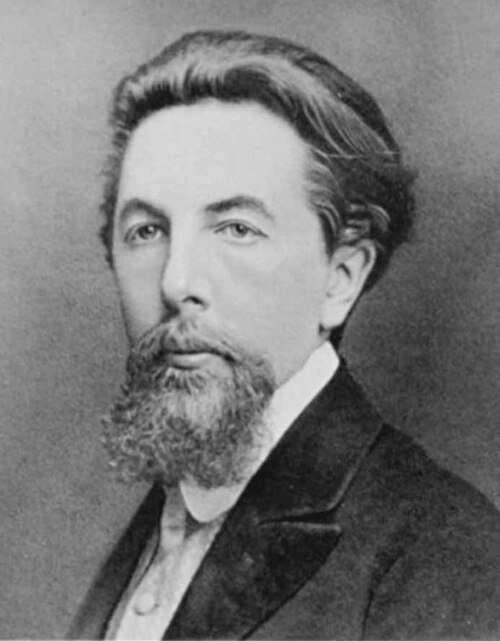
\includegraphics[width=\linewidth]{images/book3/tsvet.jpg}
\end{minipage}\hfill
\begin{minipage}[t]{0.78\linewidth}
\vspace{0pt}
Le botaniste Mikhaïl Tsvet versa un extrait de feuilles vertes dans un tube de verre rempli de craie en
poudre et l'entraîna avec un solvant~: les pigments se séparèrent en bandes colorées, chlorophylles vertes
et caroténoïdes jaunes. En 1906, il nomma la méthode \omterm{def:b2:chromatography:principle}{chromatographie}, «~écriture des couleurs~». Elle fut
largement ignorée pendant un quart de siècle, jusqu'à ce qu'on la reprenne pour les produits naturels
dans les années 1930. (Portrait~: auteur inconnu, domaine public~; Wikimedia Commons.)
\end{minipage}
\end{history}

\begin{safety}{\ghs[5mm]{GHS02}\,\ghs[5mm]{GHS05}\,\ghs[5mm]{GHS06}\,\ghs[5mm]{GHS07}\,\ghs[5mm]{GHS08}\,\ghs[5mm]{GHS09}}
L'acétonitrile et le méthanol, constituants organiques habituels des \omterm{def:b2:chromatography:principle}{phases mobiles} de CLHP, sont
inflammables et toxiques~; l'hexane, utilisé en \omterm{def:b2:chromatography:principle}{chromatographie} sur colonne, est inflammable, dangereux
pour la santé et toxique pour les organismes aquatiques. Les déchets de solvant sont collectés, jamais
versés à l'évier.
% ledger: ghs:acetonitrile, ghs:methanol, ghs:hexane
\end{safety}

\section{Exercices}

\begin{exercise}[$\star$]\label{exo:b2:chromatography:1}
Un composé a $t_R = \qty{5.0}{min}$ sur une colonne dont le \omterm{def:b2:chromatography:retention}{temps mort} vaut \qty{1.0}{min}. Calculer son
\omterm{def:b2:chromatography:retention}{facteur de rétention} et la fraction de son temps passée dans la \omterm{def:b2:chromatography:principle}{phase mobile}.
\end{exercise}

\begin{exercise}[$\star$]\label{exo:b2:chromatography:2}
Un pic à $t_R = \qty{6.0}{min}$ a une largeur à la base de \qty{0.30}{min}. Calculer le \omterm{def:b2:chromatography:plates}{nombre de plateaux}.
\end{exercise}

\begin{exercise}[$\star$]\label{exo:b2:chromatography:3}
Une colonne de \qty{250}{mm} donne $N = 10\,000$ pour un composé. Calculer la \omterm{def:b2:chromatography:plates}{hauteur de plateau}.
\end{exercise}

\begin{exercise}[$\star$]\label{exo:b2:chromatography:4}
CPG ou CLHP~? L'éthanol dans le sang~; une protéine~; la caféine dans une boisson~; le benzène dans l'essence~; les sucres dans un jus de fruit.
\end{exercise}

\begin{exercise}[$\star\star$]\label{exo:b2:chromatography:5}
Deux pics~: $t_{R1} = \qty{4.0}{min}$, $w_1 = \qty{0.40}{min}$~; $t_{R2} = \qty{4.6}{min}$, $w_2 =
\qty{0.50}{min}$. Calculer la \omterm{def:b2:chromatography:separation}{résolution}. Sont-ils séparés à la ligne de base~?
\end{exercise}

\begin{exercise}[$\star\star$]\label{exo:b2:chromatography:6}
Combien de plateaux faut-il pour séparer deux composés avec $\alpha = 1.10$ et $k_2 = 4.0$ à
$R_s = 1.5$~?
\end{exercise}

\begin{exercise}[$\star\star$]\label{exo:b2:chromatography:7}
Une colonne a $A = \qty{5}{\micro m}$, $B = \qty{8}{\micro m.mm/s}$, $C = \qty{2}{\micro m.s/mm}$
(données de l'exercice). Trouver la vitesse optimale et la plus petite \omterm{def:b2:chromatography:plates}{hauteur de plateau}.
\end{exercise}

\begin{exercise}[$\star\star$]\label{exo:b2:chromatography:8}
Prévoir l'ordre d'\omterm{def:b2:chromatography:principle}{élution} du benzène, du phénol et du toluène en CLHP en \omterm{def:b2:chromatography:techniques}{phase inverse} avec une \omterm{def:b2:chromatography:principle}{phase
mobile} eau--méthanol, et ce qui se passe quand on augmente la fraction de méthanol.
\end{exercise}

\begin{exercise}[$\star\star$]\label{exo:b2:chromatography:9}
Une solution d'étalonnage d'un analyte à \qty{20.0}{mg/L}, avec l'\omterm{def:b2:chromatography:quantitative}{étalon interne} à \qty{10.0}{mg/L},
donne les aires 860 et 400. Un échantillon additionné d'étalon à \qty{10.0}{mg/L} donne les aires 645 et
410. Calculer le \omterm{def:b2:chromatography:quantitative}{facteur de réponse} et la concentration de l'analyte (données de l'exercice).
\end{exercise}

\begin{exercise}[$\star\star\star$]\label{exo:b2:chromatography:10}
Une séparation donne $R_s = 1.06$. Quelle longueur de colonne, rapportée à la longueur actuelle, donne $R_s = 1.5$, et
que coûte-t-elle en temps~? De quels autres leviers dispose-t-on~?
\end{exercise}

\begin{exercise}[$\star\star\star$]\label{exo:b2:chromatography:11}
Pour deux pics gaussiens de même hauteur et de même largeur, de largeur à la base $w = 4\sigma$, calculer
le signal à mi-chemin entre eux, rapporté à la hauteur des pics, pour $R_s = 1$ et pour $R_s = 1.5$
(négliger la contribution du pic éloigné à chaque maximum).
\end{exercise}

\begin{exercise}[$\star\star\star$]\label{exo:b2:chromatography:12}
À $N$ et $\alpha$ constants, comparer le facteur de \omterm{def:b2:chromatography:separation}{résolution} $k_2/(1+k_2)$ et la durée relative
d'analyse $1 + k_2$ pour $k_2 = 2$, 5 et 10. Quel domaine de $k$ choisir~?
\end{exercise}

\section{Problème~: la caféine d'une boisson énergisante}

\begin{problem}[{Problème du week-end --- l'ordre d'élution en phase inverse, les performances d'une
colonne d'après un chromatogramme, l'amélioration de la séparation, et le dosage par étalon interne}]
\label{pb:b2:chromatography:1}
Données de l'exercice (inventées, il ne s'agit pas d'une méthode réelle). Une boisson énergisante est
diluée dix fois (\qty{5.00}{mL} portés à
\qty{50.0}{mL}) et l'on ajoute de la théophylline comme \omterm{def:b2:chromatography:quantitative}{étalon interne}, à \qty{40.0}{mg/L} dans la
solution diluée. Colonne~: \qty{150}{mm}, \omterm{def:b2:chromatography:techniques}{phase inverse}~; \omterm{def:b2:chromatography:principle}{phase mobile} eau--méthanol~; détection UV. La
matrice non retenue (sucres et sels) sort à $t_M = \qty{1.0}{min}$~; la théophylline à
\qty{3.0}{min} (largeur à la base \qty{0.18}{min})~; la caféine à \qty{3.4}{min} (largeur à la base \qty{0.20}{min}).
Étalonnage~: caféine à \qty{50.0}{mg/L} et théophylline à \qty{40.0}{mg/L} donnent les aires 1500 et
1000. Échantillon~: aires 970 (caféine) et 1010 (théophylline). Une canette contient \qty{250}{mL}.
% ledger: ghs:caffeine, ghs:methanol

\begin{center}
\begin{tikzpicture}
\begin{axis}[width=0.75\linewidth, height=4.4cm, xmin=0, xmax=5, ymin=0, ymax=1,
  xlabel={temps (min)}, ylabel={absorbance (u.a.)}, label style={font=\small},
  tick label style={font=\scriptsize}, ytick=\empty]
\addplot[omDef, thick] table[x=t, y=s] {figdata/out/bachelor-2-chromatogram-c.dat};
\node[font=\scriptsize] at (axis cs:1.0,0.42) {matrice};
\node[font=\scriptsize] at (axis cs:2.62,0.86) {théophylline};
\node[font=\scriptsize] at (axis cs:3.85,0.84) {caféine};
\end{axis}
\end{tikzpicture}
\end{center}
% figdata: bachelor-2/chromatogram.py part c

\medskip
\noindent\textbf{Partie I --- \omterm{def:b2:chromatography:techniques}{Phase inverse}.}
\begin{enumerate}
  \item Décrire les \omterm{def:b2:chromatography:principle}{phases stationnaire} et mobile d'une colonne en \omterm{def:b2:chromatography:techniques}{phase inverse}.
  \item Pourquoi les sucres sortent-ils au \omterm{def:b2:chromatography:retention}{temps mort}~?
  \item La caféine est la 1,3,7-triméthylxanthine, la théophylline la 1,3-diméthylxanthine. Expliquer leur
        ordre d'\omterm{def:b2:chromatography:principle}{élution}.
  \item Pourquoi la théophylline est-elle ici un bon \omterm{def:b2:chromatography:quantitative}{étalon interne}~?
  \item Qu'arriverait-il aux deux \omterm{def:b2:chromatography:retention}{temps de rétention} si l'on augmentait la fraction de méthanol~?
  \item Que mesure le \omterm{def:b2:chromatography:retention}{temps mort}~?
\end{enumerate}

\medskip
\noindent\textbf{Partie II --- Performances de la colonne.}
\begin{enumerate}[resume]
  \item Calculer les \omterm{def:b2:chromatography:retention}{facteurs de rétention} de la théophylline et de la caféine.
  \item Calculer le \omterm{def:b2:chromatography:separation}{facteur de sélectivité}.
  \item Calculer le \omterm{def:b2:chromatography:plates}{nombre de plateaux} pour la caféine et pour la théophylline.
  \item Calculer la \omterm{def:b2:chromatography:plates}{hauteur de plateau} pour la caféine.
  \item Calculer la \omterm{def:b2:chromatography:separation}{résolution} entre les deux pics.
  \item La vérifier à l'aide de l'équation de la \omterm{def:b2:chromatography:separation}{résolution}.
  \item Les pics sont-ils séparés à la ligne de base~?
\end{enumerate}

\medskip
\noindent\textbf{Partie III --- Plus vite ou mieux.}
\begin{enumerate}[resume]
  \item Pour gagner du temps, on raccourcit la colonne à \qty{75}{mm} (même garnissage, même débit). Que
        devient la \omterm{def:b2:chromatography:separation}{résolution}~?
  \item Et la durée de l'analyse~?
  \item Que donnerait au contraire une colonne de \qty{300}{mm}, et à quel prix~?
  \item Quel levier agit sur $\alpha$~?
  \item Augmenter $k$ aiderait-il beaucoup ici~?
\end{enumerate}

\medskip
\noindent\textbf{Partie IV --- Dosage.}
\begin{enumerate}[resume]
  \item Calculer le \omterm{def:b2:chromatography:quantitative}{facteur de réponse} de la caféine par rapport à la théophylline.
  \item Pourquoi le volume injecté n'importe-t-il pas~?
  \item Calculer la concentration de la caféine dans la solution diluée.
  \item Calculer la concentration de la caféine dans la boisson.
  \item Que se passerait-il si un composé de la matrice était coélué avec la théophylline~?
  \item Qu'exigerait au contraire un étalonnage externe~?
  \item Donner la masse de caféine contenue dans une canette de \qty{250}{mL}.
\end{enumerate}
\end{problem}
